%!TEX root = ../document.tex

\section[Final Prototype (Author: Fabian Tschirschnitz)]{Final Prototype}
\label{sec:FINAL_PROTOTYPE}
Our final prototype, including all feedback we gained through user testing, is a mock-up for an Eclipse plugin that addresses the observed needs of database developers. Figure \ref{fig:final_prototype_overview} illustrates a potential interface of our final revision.
\begin{figure}
\begin{centering}
    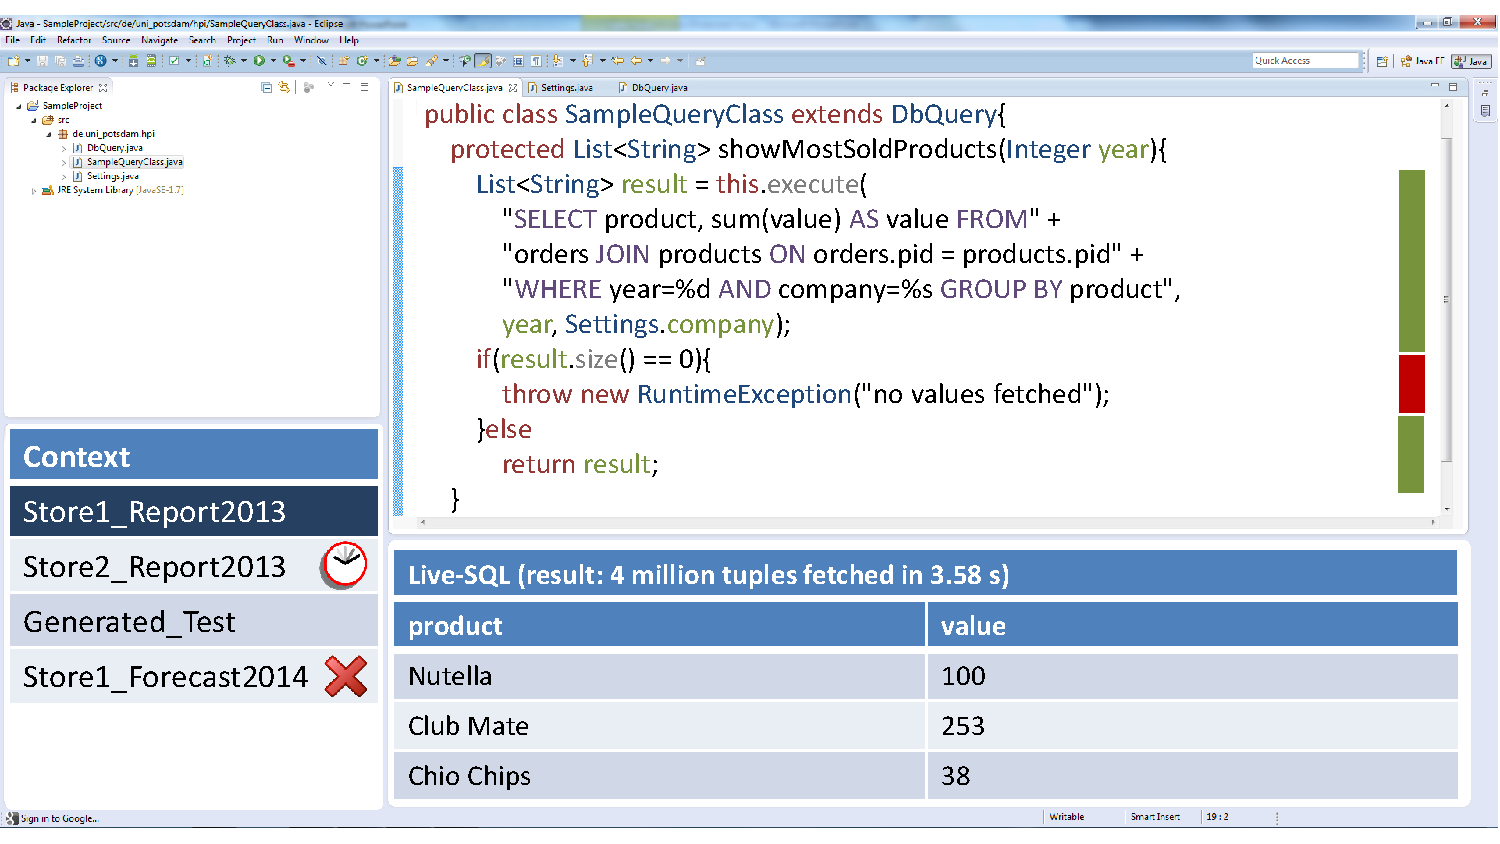
\includegraphics[width=1.0\linewidth]{images/final_prototype}
    \caption{Overview of the final prototype}
    % #selfrespect
    \label{fig:final_prototype_overview}
\end{centering}
\end{figure}
The UI mainly consists of the following three parts:
\begin{description}
	\item [Code Editor] The \emph{Code Editor} builds on top of the standard Eclipse built-in editor, with some added enhancements like syntax highlighting for inline SQL statements and an instant indications for code coverage, which can be seen on the right side of the editor's pane. The latter visualizes the code branches that will be executed depending on the currently selected data context.
	\item [Live-SQL] In the \emph{Live-SQL} frame on the bottom of the IDE, the developer gets instant data access to the underlying database tables and views. It is also possible to explore the result sets of sub-queries. Furthermore, the data is fortified with runtime information and data heuristics. %We will as you can see later.
	\item [Context Browser] The \emph{Context Browser} allows the developer to navigate through different data contexts. Some contexts ask for special attention from the programmer, e.g. those evoking errors or slowing down runtime, and are highlighted by an icon appearing next to their names. %check ob das mit dem icon noch so stimmt.
\end{description}
In the following section we lay down the main features of the customized IDE and how the user can easily interact with this new environment.\\
In order to always provide the programmer with all available Data Context, our solution focuses on instant and easy access to the underlying database at any time. When the the developer selects a table, view, or sub-select in his SQL-statement our IDE responds with an immediate preview of the corresponding data, illustrated in Figure \ref{fig:final_prototype_instant}. Furthermore the system displays meaningful visualizations of the data to give hints on performance issues, e.g. the size and the fetch time of the relation. Note how this approach not only allows for a permanent connection between code and Data Contexts but also dispenses with any workflow interruptions as they often appear in nowadays solutions. Therefore our solution allows for a highly comfortable development process.\\
\begin{figure}
\begin{centering}
    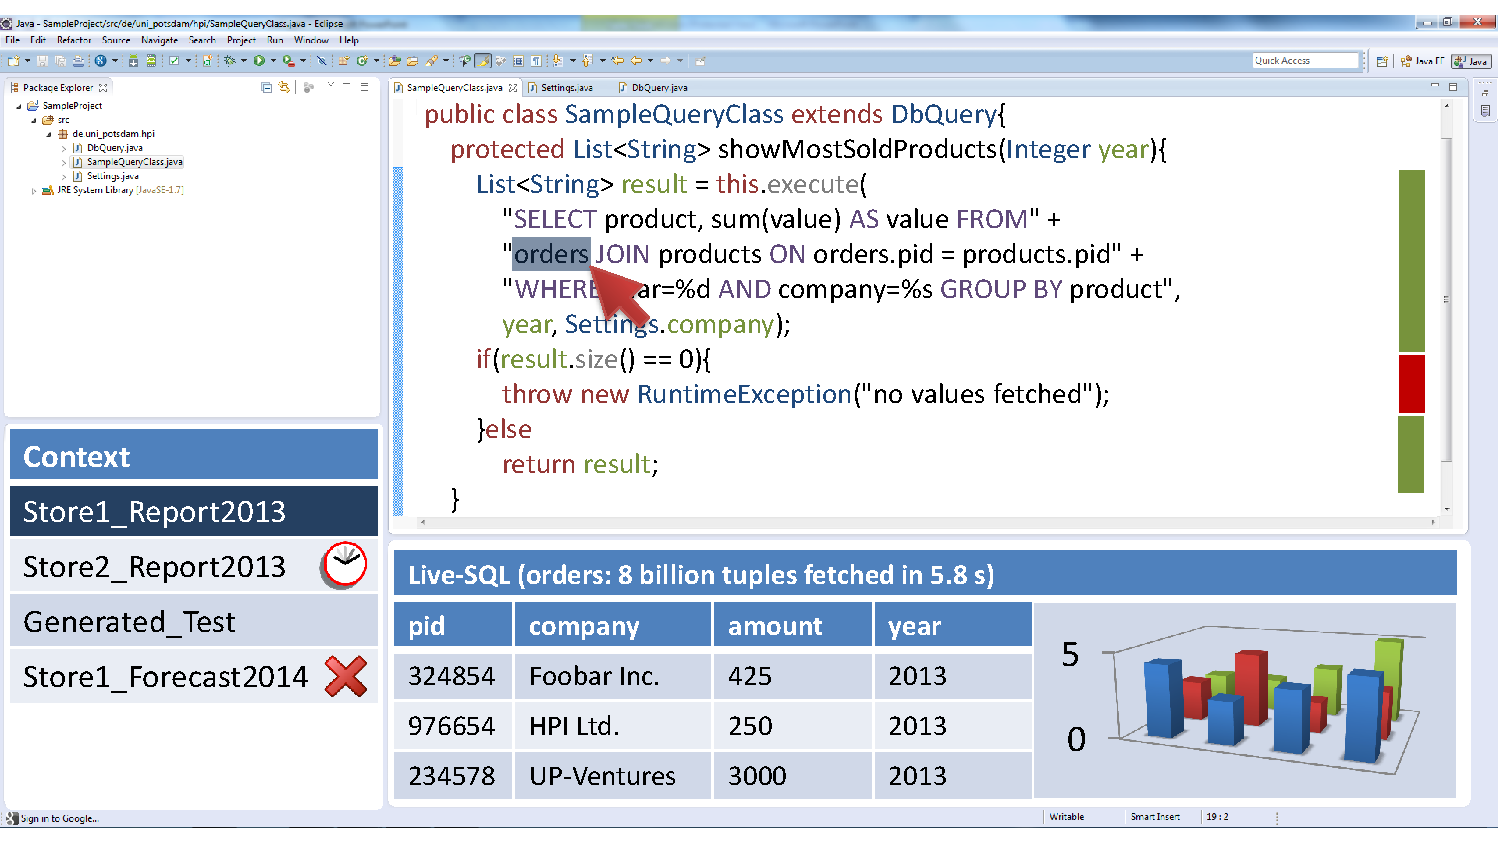
\includegraphics[width=1.0\linewidth]{images/instant}
    \caption{Instant data inspection of relations and sub-queries}
    % #selfrespect
    \label{fig:final_prototype_instant}
\end{centering}
\end{figure}
In the Context Browser little icons highlight salient contexts, such as \emph{Store2\_Report2013} in Figure \ref{fig:final_prototype_slow}. The little alarm clock behind the context name suggests that this context might perform comparatively slow during runtime and therefore reminds the developer to fix the issue. To investigate, the developer selects the context in the browser and gets immediate feedback in the Live-SQL pane at the bottom, where he realizes that the result relation takes relatively long time to be fetched. As a response he now could adapt the SQL-statement towards the output intended by the overlying method (see the red highlighted code in Figure \ref{fig:final_prototype_slow}). After the developer has changed the code in the editor pane, the Live-SQL viewer displays a \emph{diff} to the result relation before the code change. If the adjusted query decreases its fetch time by a high enough amount, the clock symbol in the Context Browser will disappear and the issue is solved.\\
\begin{figure}
\begin{centering}
    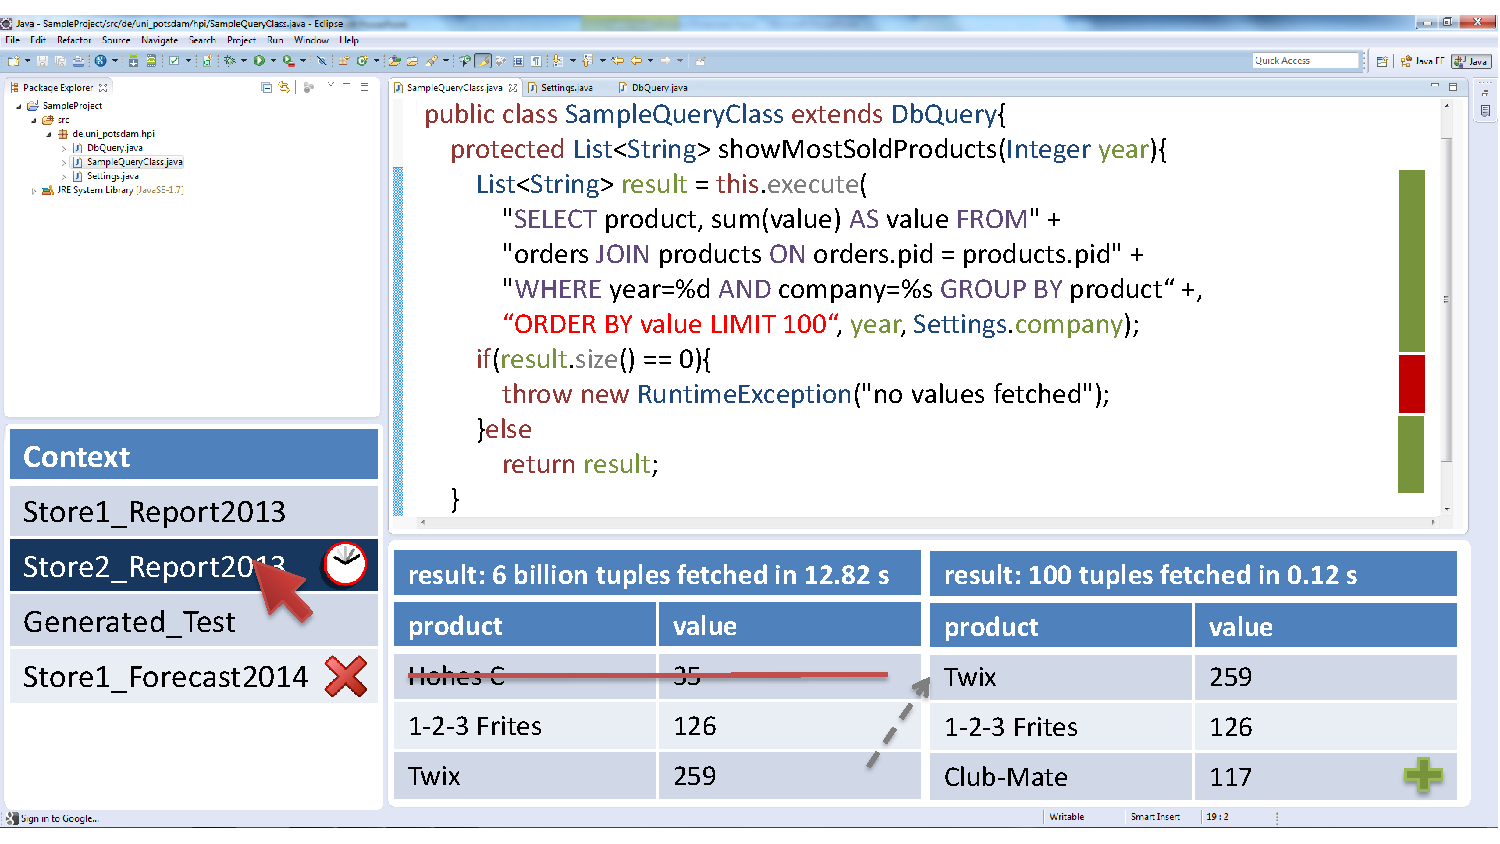
\includegraphics[width=1.0\linewidth]{images/slow}
    \caption{Performance flaw indication}
    % #selfrespect
    \label{fig:final_prototype_slow}
\end{centering}
\end{figure}
Due to the fact that a Data Context in our proposed system is not only a database state but also presents runtime information of the code, we are also able to warn the developer about error states his software might run into for certain input combinations. Such an exceptional runtime context is displayed in Figure \ref{fig:final_prototype_error}, namely \emph{Store1\_Forecast2014}. Here, the result set is empty, which directly influences the surrounding code of the query. To inform the user, the covered branches are marked differently than in the previous examples. Because of the zero fetched rows a runtime error is thrown in the method, indicated by the red cross icon in the Context Browser. The variable that causes this faulty branch execution is the method's parameter \emph{year}, made obvious by red background coloring for this word. Hovering over this variable provides the programmer with the actual value to support him or her understand the reason that caused the issue. Going from here, the developer can alternatively adapt the value of the input variable or mock the result data by inserting tuples in the Live-SQL tab for this particular result set, which would force another branch execution.\\
\begin{figure}
\begin{centering}
    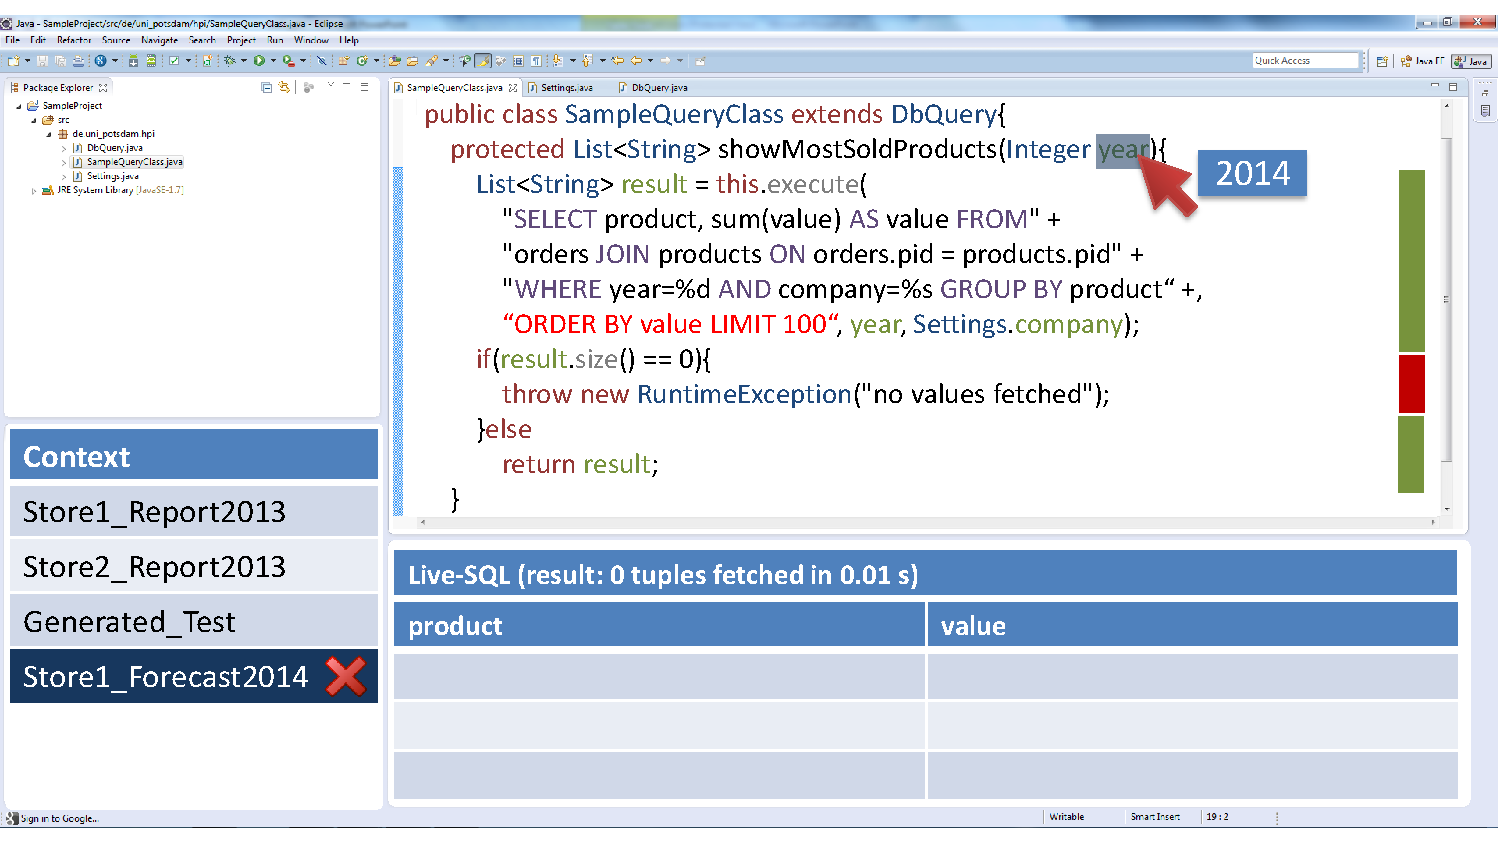
\includegraphics[width=1.0\linewidth]{images/error}
    \caption{Runtime-error indication and code coverage}
    % #selfrespect
    \label{fig:final_prototype_error}
\end{centering}
\end{figure}